%% This is file `DEMO-TUDaThesis.tex' version 3.32 (2023/06/19),
%% it is part of
%% TUDa-CI -- Corporate Design for TU Darmstadt
%% ----------------------------------------------------------------------------
%%
%%  Copyright (C) 2018--2023 by Marei Peischl <marei@peitex.de>
%%
%% ============================================================================
%% This work may be distributed and/or modified under the
%% conditions of the LaTeX Project Public License, either version 1.3c
%% of this license or (at your option) any later version.
%% The latest version of this license is in
%% http://www.latex-project.org/lppl.txt
%% and version 1.3c or later is part of all distributions of LaTeX
%% version 2008/05/04 or later.
%%
%% This work has the LPPL maintenance status `maintained'.
%%
%% The Current Maintainers of this work are
%%   Marei Peischl <tuda-ci@peitex.de>
%%   Markus Lazanowski <latex@ce.tu-darmstadt.de>
%%
%% The development respository can be found at
%% https://github.com/tudace/tuda_latex_templates
%% Please use the issue tracker for feedback!
%%
%% If you need a compiled version of this document, have a look at
%% http://mirror.ctan.org/macros/latex/contrib/tuda-ci/doc
%% or at the documentation directory of this package (if installed)
%% <path to your LaTeX distribution>/doc/latex/tuda-ci
%% ============================================================================
%%
% !TeX program = lualatex
%%

\documentclass[
	ngerman,
	ruledheaders=section,%Ebene bis zu der die Überschriften mit Linien abgetrennt werden, vgl. DEMO-TUDaPub
	class=report,% Basisdokumentenklasse. Wählt die Korrespondierende KOMA-Script Klasse
	thesis={type=master},% Dokumententyp Thesis, für Dissertationen siehe die Demo-Datei DEMO-TUDaPhd
	accentcolor=9c,% Auswahl der Akzentfarbe
	custommargins=true,% Ränder werden mithilfe von typearea automatisch berechnet
	marginpar=false,% Kopfzeile und Fußzeile erstrecken sich nicht über die Randnotizspalte
	%BCOR=5mm,%Bindekorrektur, falls notwendig
	parskip=half-,%Absatzkennzeichnung durch Abstand vgl. KOMA-Script
	fontsize=11pt,%Basisschriftgröße laut Corporate Design ist mit 9pt häufig zu klein
	%	logofile=example-image, %Falls die Logo Dateien nicht vorliegen
]{tudapub}


% Der folgende Block ist nur bei pdfTeX auf Versionen vor April 2018 notwendig
\usepackage{iftex}
\ifPDFTeX
	\usepackage[utf8]{inputenc}%kompatibilität mit TeX Versionen vor April 2018
\fi

%%%%%%%%%%%%%%%%%%%
%Sprachanpassung & Verbesserte Trennregeln
%%%%%%%%%%%%%%%%%%%
\usepackage[ngerman, main=english]{babel}
\usepackage[autostyle]{csquotes}% Anführungszeichen vereinfacht

% Falls mit pdflatex kompiliert wird, wird microtype automatisch geladen, in diesem Fall muss diese Zeile entfernt werden, und falls weiter Optionen hinzugefügt werden sollen, muss dies über
% \PassOptionsToPackage{Optionen}{microtype}
% vor \documentclass hinzugefügt werden.
\usepackage{microtype}

%%%%%%%%%%%%%%%%%%%
%Literaturverzeichnis
%%%%%%%%%%%%%%%%%%%
\usepackage{biblatex}   % Literaturverzeichnis
%\bibliography{DEMO-TUDaBibliography.bib}
\addbibresource{biblio.bib}
\setcounter{tocdepth}{4}
\setcounter{secnumdepth}{4}


%%%%%%%%%%%%%%%%%%%
%Paketvorschläge Tabellen
%%%%%%%%%%%%%%%%%%%
%\usepackage{array}     % Basispaket für Tabellenkonfiguration, wird von den folgenden automatisch geladen
\usepackage{tabularx}   % Tabellen, die sich automatisch der Breite anpassen
%\usepackage{longtable} % Mehrseitige Tabellen
%\usepackage{xltabular} % Mehrseitige Tabellen mit anpassbarer Breite
\usepackage{booktabs}   % Verbesserte Möglichkeiten für Tabellenlayout über horizontale Linien
\usepackage{float}
\usepackage{amsmath}

%%%%%%%%%%%%%%%%%%%
%Paketvorschläge Mathematik
%%%%%%%%%%%%%%%%%%%
%\usepackage{mathtools} % erweiterte Fassung von amsmath
%\usepackage{amssymb}   % erweiterter Zeichensatz
%\usepackage{siunitx}   % Einheiten

%Formatierungen für Beispiele in diesem Dokument. Im Allgemeinen nicht notwendig!
\let\file\texttt
\let\code\texttt
\let\tbs\textbackslash
\let\pck\textsf
\let\cls\textsf

\usepackage{pifont}% Zapf-Dingbats Symbole
\newcommand*{\FeatureTrue}{\ding{52}}
\newcommand*{\FeatureFalse}{\ding{56}}

\begin{document}

\Metadata{
	title=Thesis,
	author=Denis Andrić
}

\title{Implementation of Neural Models for Accurate Prediction of Robot Trajectories in Hamiltonian Spaces: A Graph Neural Network Approach}
\subtitle{Implementierung von neuronalen Modellen zur präzisen Vorhersage von Trajektorien in Hamiltonschen Räumen: 
	Ein Ansatz mit Graph-Neuronalen Netzwerken}
\author[D. Andrić]{Denis Andrić}
\studentID{2486004}%optionales Argument ist die Signatur,
\birthplace{Darmstadt}%Geburtsort, bei Dissertationen zwingend notwendig
\reviewer{Georgia Chalvatzaki \and An Thai Le}%Gutachter

%Diese Felder werden untereinander auf der Titelseite platziert.
%\department ist eine notwendige Angabe, siehe auch dem Abschnitt `Abweichung von den Vorgaben für die Titelseite'
%\department{ce} % Das Kürzel wird automatisch ersetzt und als Studienfach gewählt, siehe Liste der Kürzel im Dokument.
%\institute{FB 20}
\addTitleBoxLogo*{
\includegraphics[width=0.5\linewidth]{logos/CELogo.png}}
\addTitleBoxLogo*{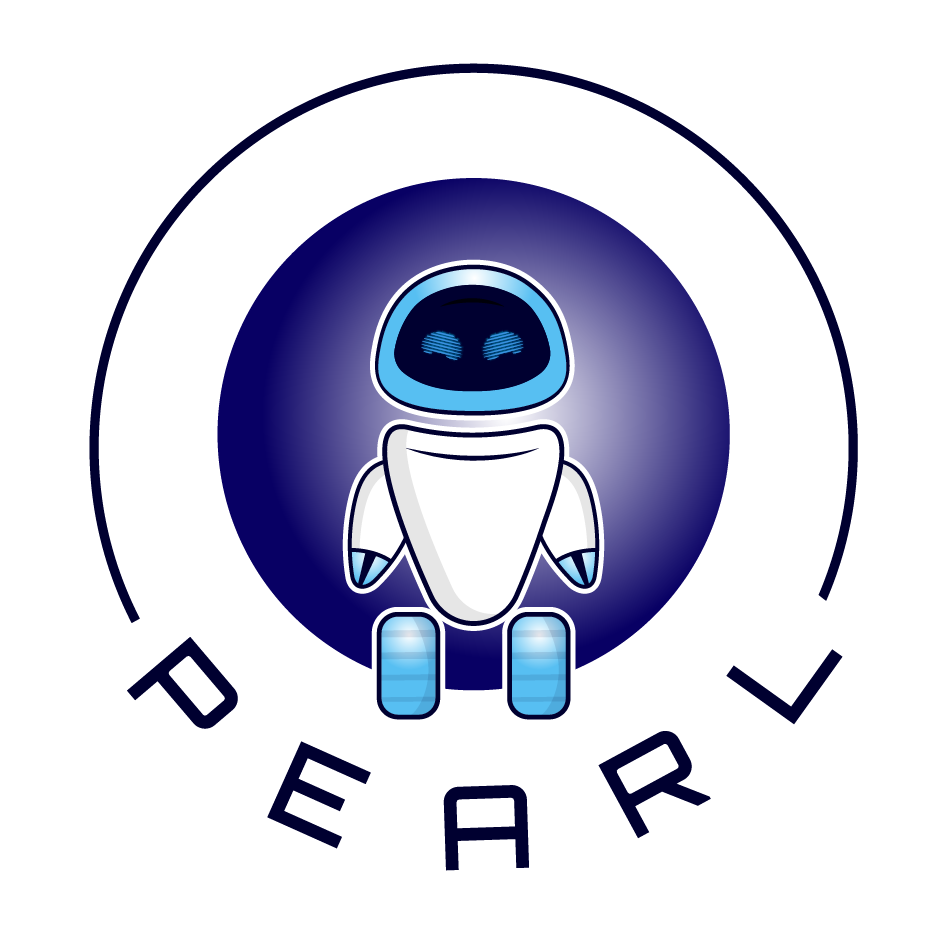
\includegraphics[width=0.5\linewidth]{logos/pearllogo.png}}
\addTitleBoxLogo*{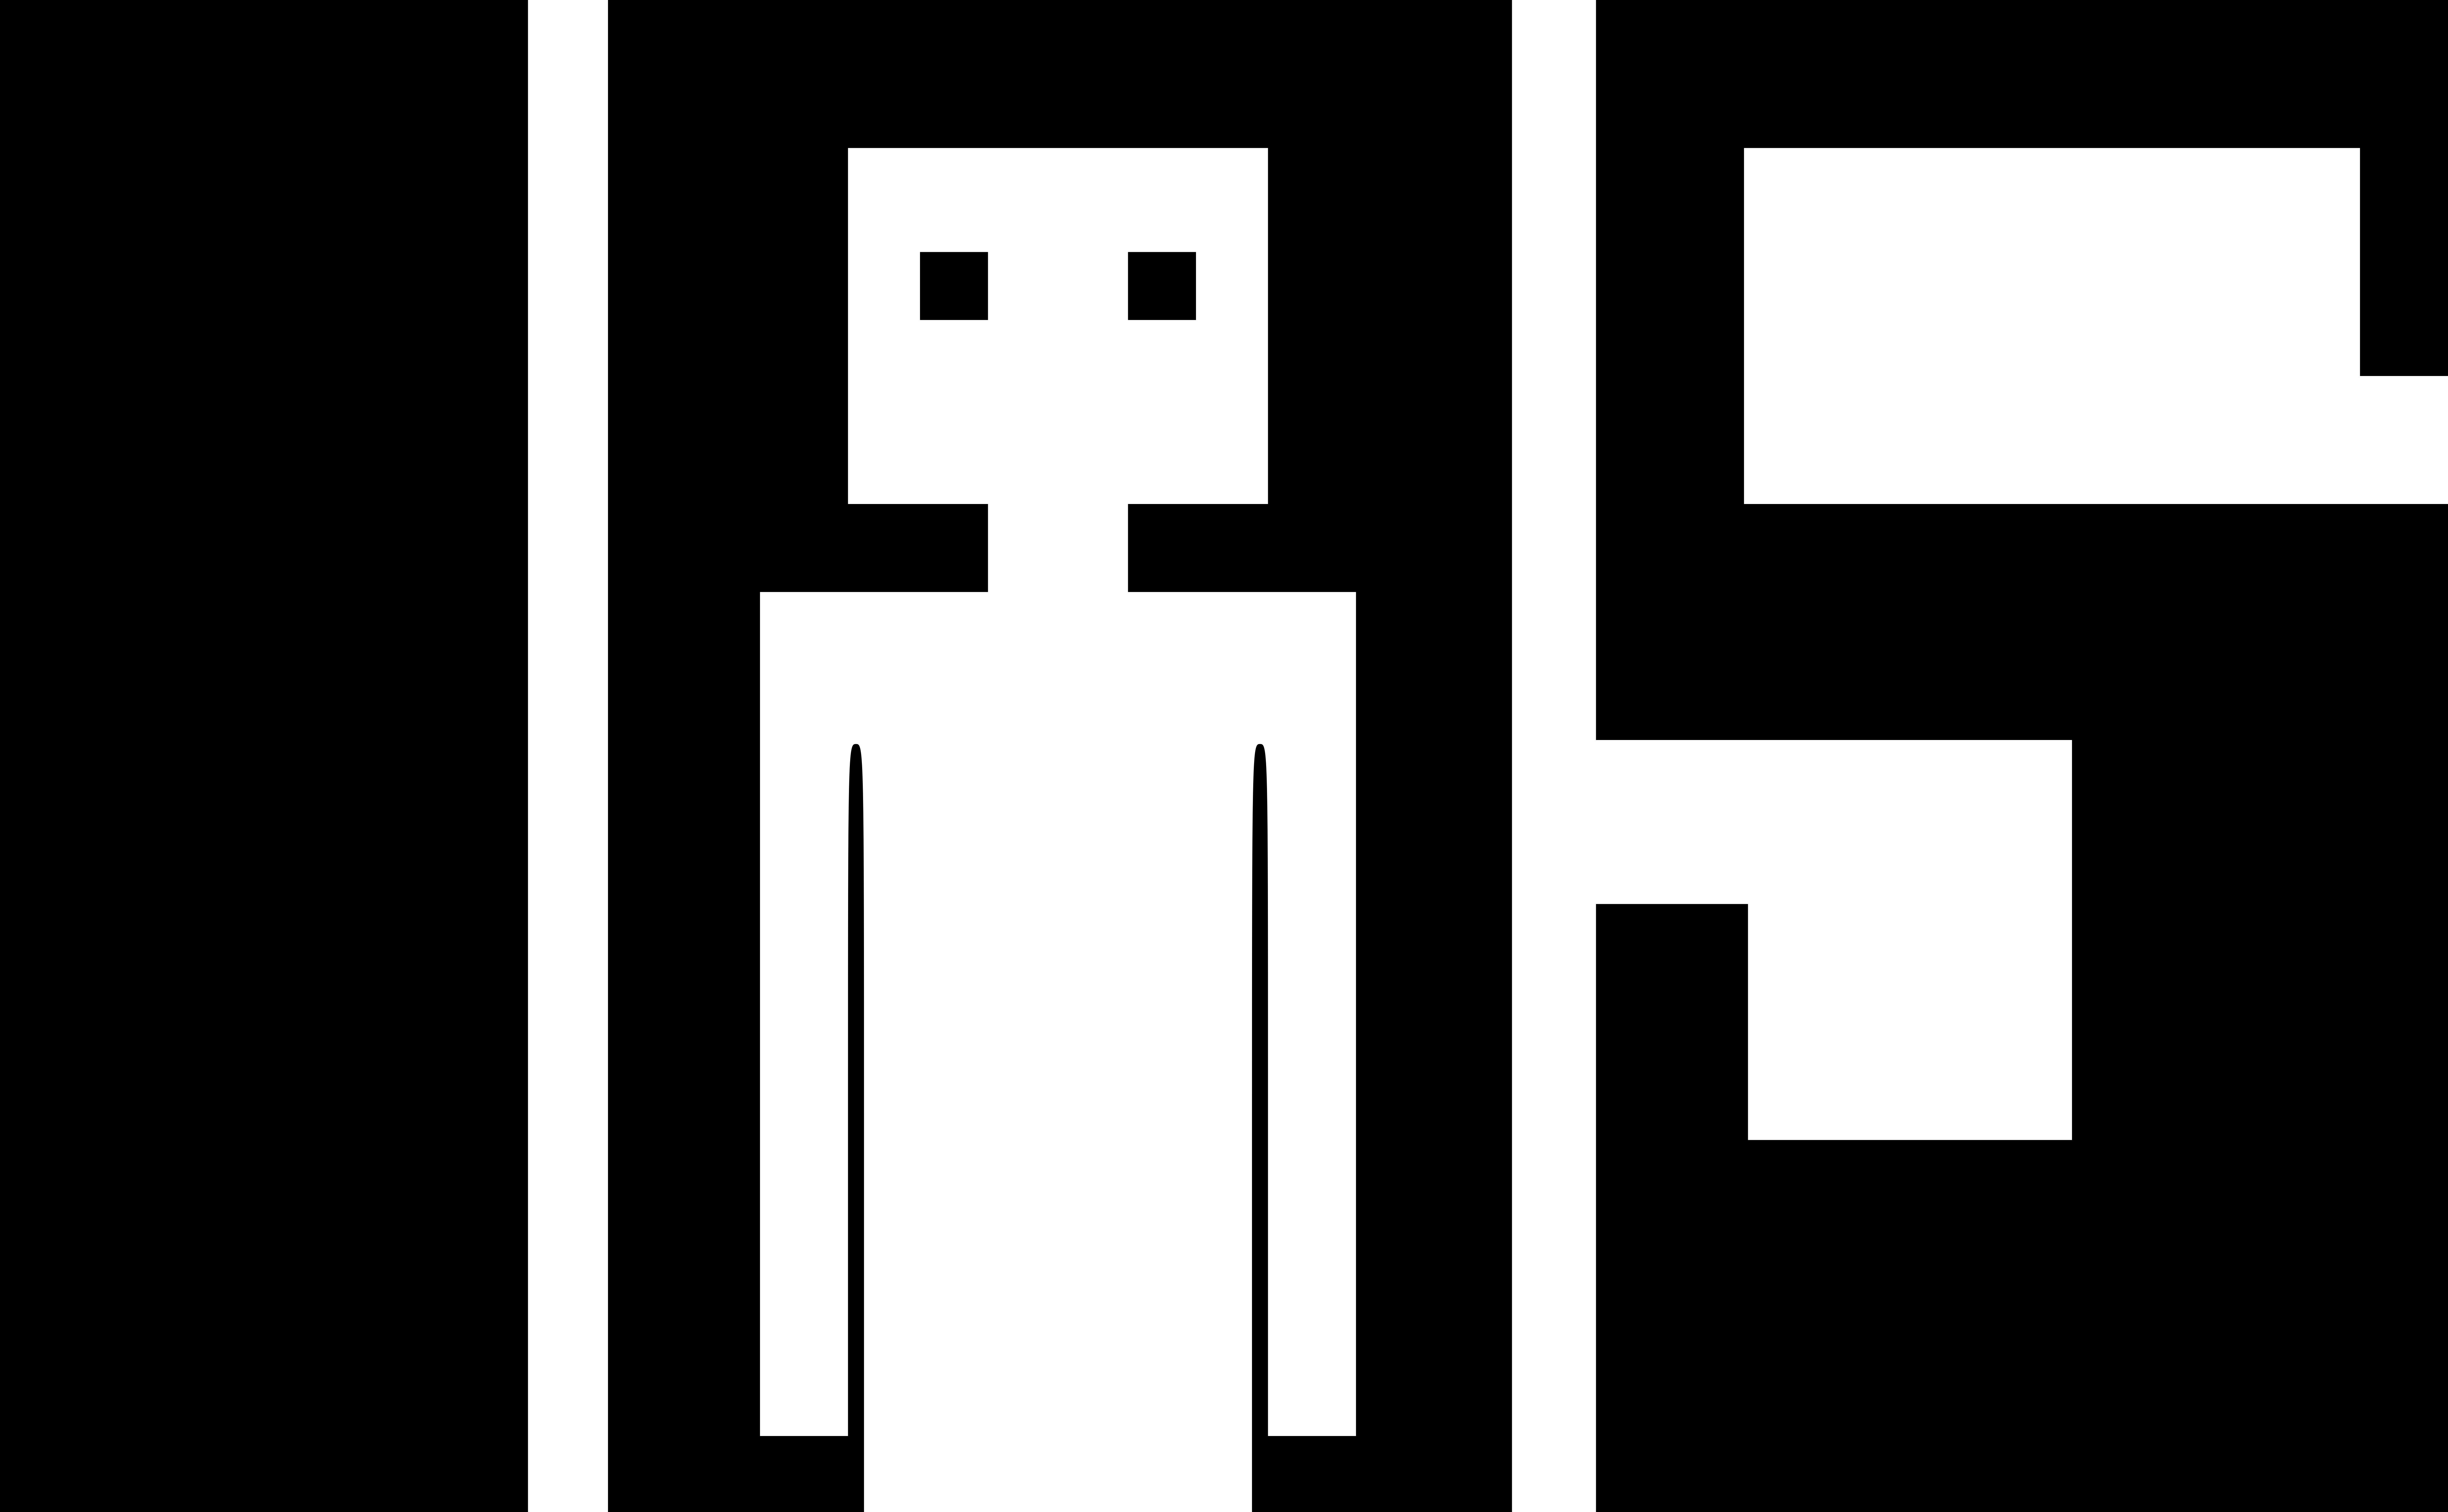
\includegraphics[width=0.5\linewidth]{logos/iasLogo.png}}
\submissiondate{\today}
\examdate{\today}

% Hinweis zur Lizenz:
% TUDa-CI verwendet momentan die Lizenz CC BY-NC-ND 2.0 DE als Voreinstellung.
% Die TU Darmstadt hat jedoch die Empfehlung von dieser auf die liberalere
% CC BY 4.0 geändert. Diese erlaubt eine Verwendung bearbeiteter Versionen und
% die kommerzielle Nutzung.
% TUDa-CI wird im nächsten größeren Release ebenfalls diese Anpassung vornehmen.
% Aus diesem Grund wird empfohlen die Lizenz manuell auszuwählen.
%\tuprints{urn=XXXXX,printid=XXXX,year=2022,license=cc-by-4.0}
% To see further information on the license option in English, remove the license= key and pay attention to the warning & help message.

% \dedication{Für alle, die \TeX{} nutzen.}

\maketitle

\affidavit
% Es gibt mit Version 3.20 die Möglichkeit ein Bild als Signatur einzubinden.
% TUDa-CI kann nicht garantieren, dass dies zulässig ist oder eine eigenhändige Unterschrift ersetzt.
% Dies ist durch Studierende vor der Verwendung abzuklären.
% Die Verwendung funktioniert so:
%\affidavit[signature-image={\includegraphics[width=\width,height=1cm]{example-image}}, <hier können andere Optionen zusätzlich stehen>]

\tableofcontents
\listoffigures
\listoftables

\chapter*{Abstract}
The introduction of the adjoint method for NeuralODEs\cite{neuralODE} has created new ways for physics-based trajectory predictions. In the subsequent chapters of this thesis, we look at deep learning models and methods targeted at predicting physical systems' behavior. We use the guiding light of Hamiltonian equations to dive into systems such as the harmonic oscillator and the three-body problem. We are intrigued with exploring graph neural networks' ability to be used in physics informed models: in the N-body problem and in the N-pendulum. This work tests the ability of graph neural networks to generalize the behavior from single realizations of elements at the node level of the graph. In this way, we hope to exemplify how such models can capture highly dynamic physical processes. 


\chapter{Introduction}
The intersection of physics and deep learning has never been more pronounced than it is today. With advancements in hardware and computational capabilities, we are now positioned to predict physical phenomena with unprecedented precision using deep learning techniques, particularly through physics-informed neural networks.\\
Physics-Informed Neural Networks (PINN) are neural networks  that encode model equations, like Partial Differential Equations (PDE), as a component of the neural network itself\cite{}. For example let us take Laplace equation which is defined as
\begin{eqnarray}
	\Delta u(\mathbf{x}) &= 0, &\texttt{   }\mathbf{x}\in \Omega,\mathbf{x}\in R^2\\
	u &= S &\texttt{   }\mathbf{x}\in \partial\Omega \text{     Dirichlet boundary condition},\\
	\frac{\partial u}{\partial \mathbf{n}} &= f(\mathbf{x}) &\texttt{   }\mathbf{x}\in \partial\Omega \text{     Neumann boundary condition}.
\end{eqnarray}
The Operator $\Delta$ is called as Laplace Operator and it defines $\Delta = \sum_i \frac{\partial^2}{\partial^2 x_i}.$\\
To build a PINN model we will use an Neural Network which will learn the solution $u$ and from that output we will calculate all needed derivatives, residuals and other parts for the optimization.

\begin{figure}[h!]
	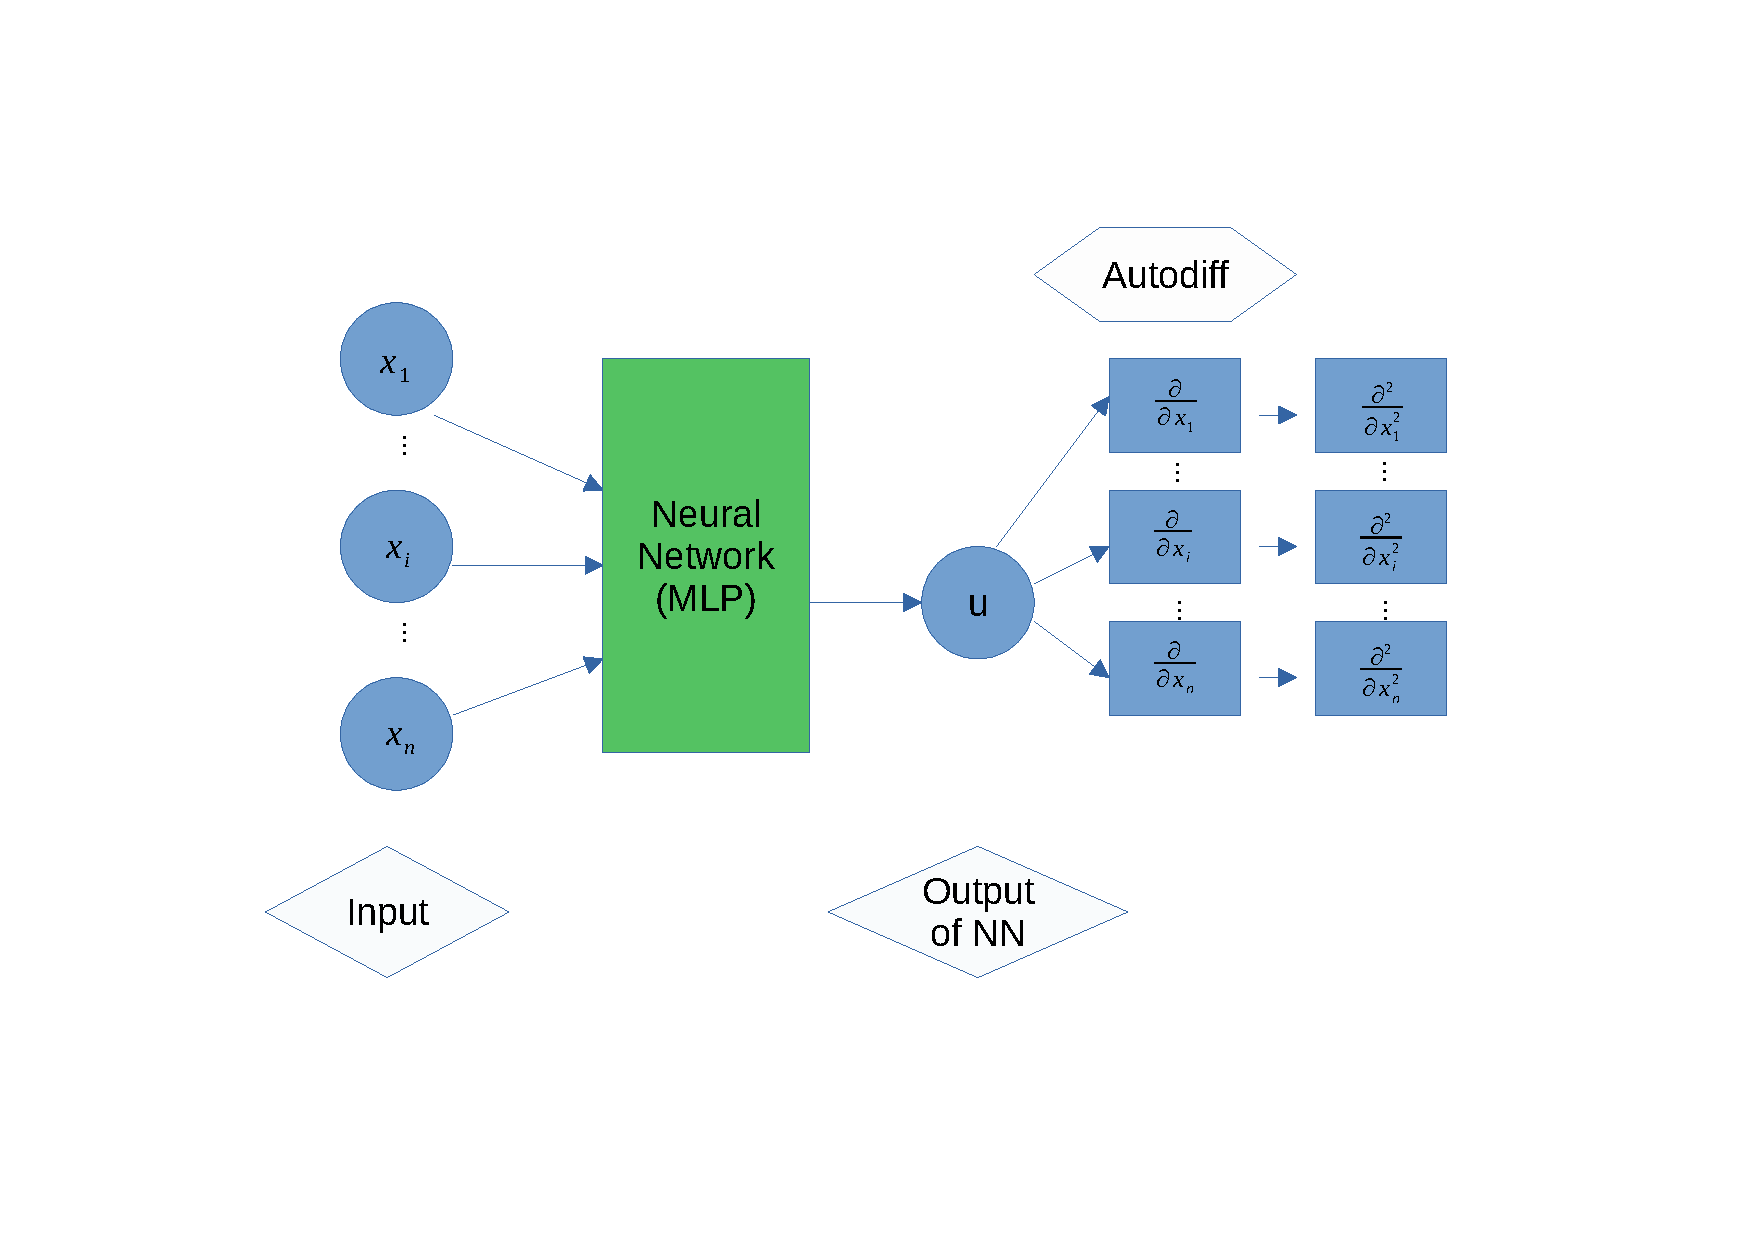
\includegraphics[width=15cm]{chapters/chapter1/pinn}
	\label{pinn}
	\caption{PINN model for Laplace Equation}
\end{figure}
In figure \ref{pinn} we can observe the architecture of such physics informed model. 
The Loss functions that we need to use to properly train our network are
\begin{eqnarray}
	\text{Loss}_s(\Theta) &=& \frac{1}{N}\sum^N_i\left(u_{\Theta}(\mathbf{x}_i)- u_i\right)^2,\\
	\text{Loss}_r(\Theta) &=& \frac{1}{R}\sum^R_i\left(\frac{\partial u_{\Theta}(\mathbf{x}_i)}{\partial x_i} - f(\mathbf{x}_i)\right)^2,\\
	\text{Loss}_l(\Theta) &=& \Delta u_{\Theta},\\
	\text{Loss}(\Theta) &=& \omega_s \text{Loss}_s +\omega_r \text{Loss}_r +\omega_l \text{Loss}_l .
\end{eqnarray}
The $\omega_s$,$\omega_r$,$\omega_l$, in this case are coefficients $0\leq \omega \leq 1$ and they are there to improve optimization capabilities which is defined as
\begin{equation}
	\Theta^* = \arg\min\text{Loss}(\Theta).
\end{equation}
The $\Theta$ are learnable parameters which can be updated with $\Theta^*$ trough optimization algorithm.\\
Such model wouldn't be possible without Automatic Differentiation\cite{} which are offered from machine learning library $\texttt{pytorch}$\cite{}. In this example we need big bunch of data and the optimization of the model could be very slow in addition if we don't have a computation capable hardware for it. Obtaining the data could be done only with exactly measurement or using some numerical solvers like FEM or Isogeometric Analysis. Don't forget, that there are Poission Equation, Wave Equation which are dependent on time $t$.\\
Those PDEs have mostly application in electrotechnical(Electro-magnetical fields) and  civil Engineering(static in construction).
In this thesis we won't work on the PDEs but similar to this topic we will try to train a model to predict the Dynamics of some physical phenomena and non-/holonomic systems of the robots.\\
The Dynamics for Robots are trivially defined as simple Second Level Ordinary Differential Equation\cite{} .
\begin{equation}
	\mathbf{M}\ddot{\mathbf{x}}(t) + \mathbf{D}(\dot{\mathbf{x}}(t)) + \mathbf{C}(\mathbf{x}(t))=0,
\end{equation} but there are other forms, as Langrange Equations of Motion if our system is holonomic\cite{}. It is based on Lagrange Function which is based on Kinetik $T$ and Potential $U$ Energy
\begin{eqnarray}
	\mathcal{L} &=& T - V,\\
	\frac{d}{dt}\frac{\partial \mathcal{L}}{\partial \dot{q}_i} - \frac{\partial \mathcal{L}}{\partial q_i}&=&0.
\end{eqnarray}   
The Lagrange Equations are used in Delan\cite{} Physics informed network and in simillar manner, but for us are most interesting to use Hamiltonian Equations of Motion.
They work for holonomic and non-holonomic systems and they are capable to build First Level Ordinary Equation
\begin{equation}
	\dot{x} = f(x,t)
\end{equation} \\
or in Hamiltonian Form where $\mathcal{H} = T + V$
\begin{equation}
	\dot{\mathbf{z}} = \mathbf{J}\frac{\partial\mathcal{H}}{\partial \mathbf{z}}
\end{equation} where $\mathbf{z}=[\mathbf{q},\mathbf{p}]^T$ and $\mathbf{J} = \begin{bmatrix}
0 & \mathbf{I}_n\\
-\mathbf{I}_n & 0
\end{bmatrix} $\\
\begin{figure}[h!]
	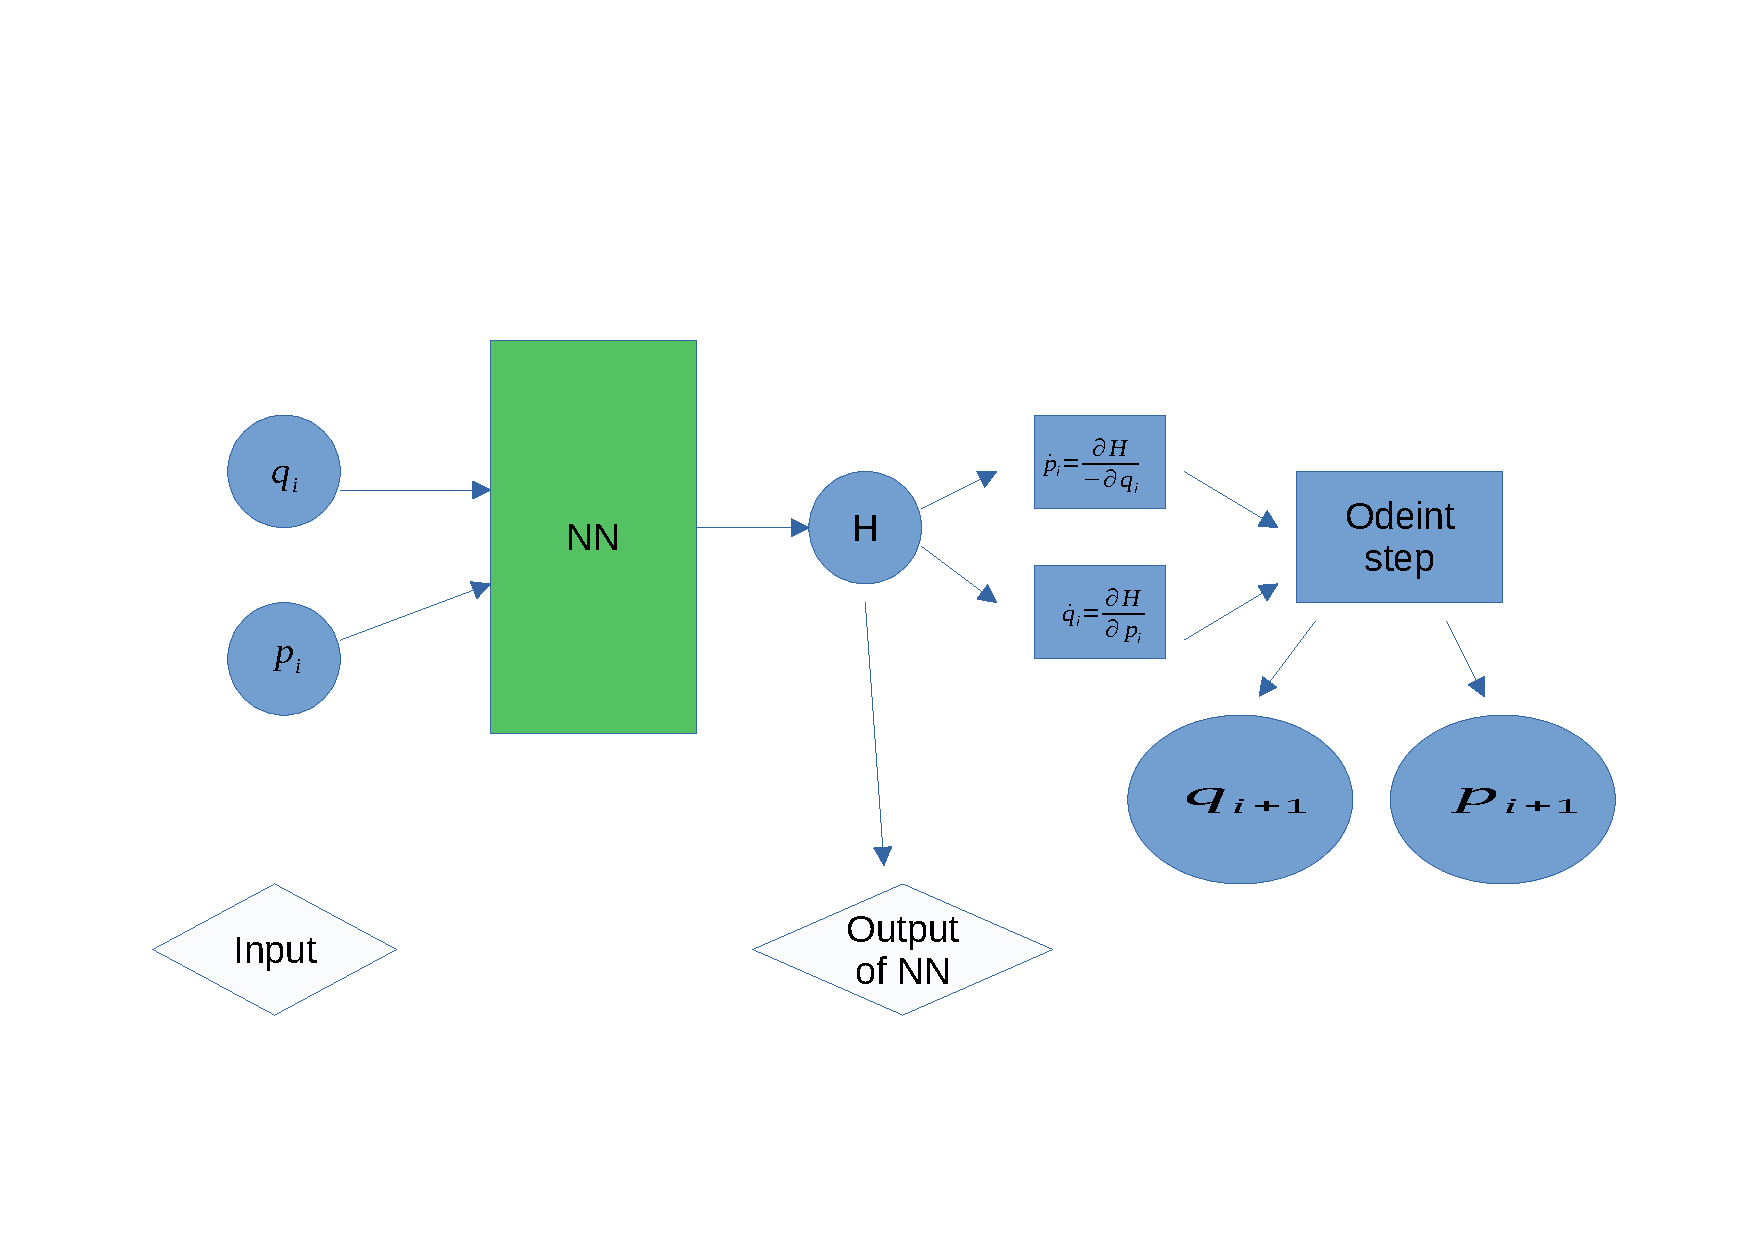
\includegraphics[width=15cm]{chapters/chapter1/hnn}
	\label{hnn}
	\caption{HNN model with integration solver step}
\end{figure}
One of such model is introduced in the \cite{} and it is called HNN. it architecture you can observe in figure \ref{hnn}.
We will make it more interesting introducing the Graph Neural Network and try to use it as a base of our architecture.\\
In this thesis we will discuss what are Hamiltonian equations and how to obtain them. In our research we stumbled upon the fact, that there are no quality datasets for training the Neural Networks which are based on physics. With this fact we brew 4 popular datasets which are based on Hamiltonian Equations of Motion.\\
Next we made new and revisit old neural architectures and test NeuralODE as new Nerual Paradigm into treaining the solutions of ODEs.\\
In the experiments we tested the capabilites of Graph Neural Networks, how do they adapt to diverse training data and their possibility to reduce or increase a degree of freedom in the training. For example how similar is the movement between 3 and 4 bodied pendulum on the same trained set of neural parameters. We hope that we will give the insight in those topics.    








%% related works, philosophy, motivations, my contributions




\printbibliography

\end{document}
